\section{Machine Learning Method}
The typical process of a machine learning classifier can be seen in Figure \ref{fig:ml_approach}. In this thesis, a supervised approach is used, which, as mentioned previously, requires labeled training data. In order to use instances, either for training or for classification, features have to be extracted, which serve as the input attributes for the classification model. In the following sections, the feature extraction process, which is depicted in Figure \ref{fig:ml_process}, is explained further.
\begin{figure}
    \centering
    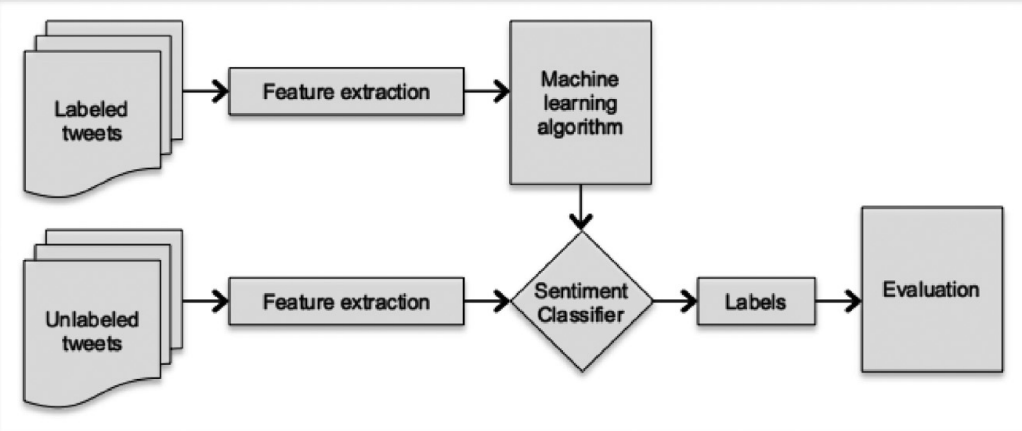
\includegraphics[scale=0.5]{Images/ML_approach.png}
    \caption{Typical process for sentiment classification by Giachanou and Crestani \cite[p.~28:3]{DBLP:journals/csur/GiachanouC16}}
    \label{fig:ml_approach}
\end{figure}


\begin{figure}
    \centering
    \tikzset{
  every shadow/.style={
    fill=none,
    shadow xshift=0pt,
    shadow yshift=0pt}
}
\tikzset{module/.append style={top color=\col,bottom color=\col}}

\smartdiagramset{uniform color list=white for 4 items,
    back arrow disabled=true, module minimum width=3cm,
    module minimum height=2cm,
    module x sep=4cm,
    text width= 3cm,
    uniform arrow color=true,
    arrow color=black,
    additions={
        additional item shape=rectangle,
        additional item offset=0.5cm,
        additional item width=3cm,
        additional item height=2cm,
        additional item text width=3cm,
        additional item fill color=white!20,
        additional item border color=black,
        additional arrow color=gray,
        additional arrow tip=stealth,
        additional arrow line width=1pt
      }
    }
    \smartdiagramadd[flow diagram:horizontal]{URL/Hashtag Removal, Stop Word Filtering, Stemming, Feature Selection}
    {below of module4/Word Frequency vs. Presence \\ Unigrams vs. Bigrams, below of module2/Dynamic vs. Static} 
    \smartdiagramconnect{->}{module4/additional-module1}
    \smartdiagramconnect{->}{module2/additional-module2}

    \vspace{25mm}

   \caption{Process for feature extraction for the machine learning method.}
    \label{fig:ml_process}
\end{figure}

\subsection{Preprocessing}
In order to prepare the tweets for feature extraction, a few steps can be taken to encounter some of the characteristics that define tweets \cite{DBLP:journals/csur/GiachanouC16}.

\subsubsection{URL/Hashtag Removal}
Tweets often contain URLs of the media, article, etc. the tweet is concerned with. Because these links in itself don't affect the sentiment, and are unique, they can be ignored to reduce data sparsity. Additionally, tweets often contain a hashtag, which indicates that the tweet is concerned with specific topic. The hashtag character "\#" is removed, to not differentiate between words such as \#good and good and thus further reduce data sparsity.

\subsubsection{Stop Word Filtering}
Common words with low impact on the sentiment of a sentence, such as "the" and "is", are referred to as stop words and can be ignored, as they do not provide any additional information. Although there are compiled lists of stop words, these often are outdated and not Twitter specific \cite{DBLP:journals/csur/GiachanouC16}. Additionally, Saif et al. observed that the usage of compiled lists reduced the accuracy of classification performance and recommended a dynamic solution, which considers the number of times a word appears over the data set \cite{data_sparsity}. This thesis combines both approaches and uses a stop word list, as well as a dynamic solution.

\subsubsection{Stemming}
Tweets as an informal message often contain misspelled or otherwise modified words \cite{DBLP:journals/csur/GiachanouC16}. Word stemming, according to Lovins, "reduces all words with the same root (or, if prefixes are left
untouched, the same stem) to a common form" \cite[p.~22]{Lovins1968DevelopmentOA}. Thus, different cases or spellings of the same word can be reduced to one common feature, which also reduces data sparsity.

\subsection{Feature Selection}
Feature selection is one of the most important parts of the classification process, as the classifier makes decision based on the features. Giachanou and Crestani identified several different possible features: (1) semantic Features, such as sentiment words and negations, which are extracted using lexicons; (2) syntactic Features, such as the presence of a word or term; (3) stylistic features, which include emoticons and punctuation; and (4) twitter-specific features, for example hashtags or the number of replies.

This thesis utilizes syntactic features, which are the most used features. Approaches here differentiate on which syntactic features to use. Some approaches look at each word of a tweet seperately, which is called the unigram model, while others combine two (bigram model) or more words (n-gram model) as a combined feature. The effectiveness of each model varies, as some, like Go et al., determined that bigrams reduced the accuracy in most cases, compared to unigrams \cite{GoBHaHua2009}, while others such as Pak and Paroubek concluded that bigrams offer the better accuracy compared to unigrams \cite{pak}. Thus, this thesis evaluates both unigrams, bigrams, and their combination, which has shown to improve accuracy further \cite{GoBHaHua2009}.

In addition, the usage of a term's frequency in a tweet varies. Some approaches utilize a binary presence, which does not differentiate whether a term appears multiple times in a sentence, while others utilize the frequency \cite{DBLP:journals/csur/GiachanouC16}. In this thesis, both approaches are considered.

\subsection{Classifiers}
\TODO{ngram}

Once the training data has been preprocessed and turned into features, the task of training the classifier models can begin. The classifiers chosen were Naive Bayes using the Gaussian distribution, Naive Bayes using the multinomial distribution, Random Forest, Logistic Regression and Support Vector Machine. Because the classifiers may have different runtimes, each classifier was first evaluated using a small subset of training data, in order to obtain a first impression of the training runtime. After this, the data size was gradually increased, until the entire data set was used, or the process became too resource intensive. Once the optimal training size was found, the parameters of each classifier were evaluated, to improve both performance and accuracy. If the performance could be improved, the training size was adjusted accordingly. Once the optimal parameters and training size were found, the classifiers were evaluated and compared. To facilitate a better comparison, the classifiers were evaluated both using their maximum training size, as well as the same minimum training size.

The following subsections explain each machine learning method in more detail.

    \subsubsection{Naive Bayes}
        Naive Bayes is a probabilistic, generative classification model, as it does not directly estimate the probability from the training data. It is based on the Bayes theorem, which is shown in Equation \eqref{eq:bayes}:
        \begin{equation}
            \label{eq:bayes}
            P(c_j|d_i) = \frac{P(c_j) * P(d_i|c_j)}{P(d_i)},
        \end{equation}
        where $c_j$ is a class label and $d_i$ is the document, in our case a tweet. \cite{DBLP:books/aw/TanSKK2019}. 
        
        Bayes theorem allows to calculate the posterior probability $P(c_j|d_i)$, which Tan et al. describe as "the probability of observing a class label $c_j$ for a data instance given its set of attribute values $d_i$" \cite[p.~418]{DBLP:books/aw/TanSKK2019}. To calculate the posterior probability, the class conditional probability $P(d_i|c_j)$ is needed, which describes the probability of observing a set of attribute values given a class. Because of this indirect calculation, Naive Bayes is a generative model. One approach to calculate the class conditional probability outlined by Tan et al. is to ''consider the fraction of training instances of a given class for every possible combination of attribute values'' \cite[p.~419]{DBLP:books/aw/TanSKK2019}. With a large number of attributes and values, this method becomes computationally infeasible due to the exponential growth of combinations \cite{DBLP:books/aw/TanSKK2019}.

        Due to this, the Naive Bayes assumption is employed to estimate the class conditional probability. Naive Bayes assumes conditional independence, which states that attribute values are only dependent on the class label and not each other. Thus, the class conditional probability can be calculated by using Equation \eqref{eq:naive_assumption}:
        \begin{equation}
            \label{eq:naive_assumption}
            P(d_i|c_j) = \prod_{t=1}^{n}P(w_{t}|c_j),
        \end{equation}
        with $d_i$ containing $n$ attributes $\{w_1,w_2,...,w_t\}$ \cite{DBLP:books/aw/TanSKK2019}.

        Furthermore, $P(d)$ remains constant for every class label $c$, so the class that maximizes Equation \eqref{eq:naive_final} is chosen: 
        \begin{equation}
            \label{eq:naive_final}
            P(c_j|d_i)\propto P(c_j)\prod_{t=1}^{n}P(w_{t}|c_j) .
        \end{equation}   
        
        $P(c_j)$ denotes the prior probability and thus the distribution of class labels, which can be obtained using prior knowledge or the training data.
        

        There are different models on how to implement the Naive Bayes assumption for text classification. In this thesis, the Gaussian Naive Bayes and Multinomial Naive Bayes are discussed. 
        
        \paragraph{Gaussian Naive Bayes} \mbox{} \\

        The Gaussian Naive Bayes assumes that numeric attributes, such as word count, are distributed according to the normal distribution, also called gaussian distribution \cite{nb_gauss}. According to Evans et al., "[the gaussian distribution] was originally developed as an approximation to the binomial distribution when the number of trials is large and the Bernoulli probability p is not close to 0 or 1". \cite[p.~143]{evans2011statistical}. It is described by two parameters, the mean $\mu$ and the standard deviation $\sigma$ \cite{evans2011statistical}. Applied to Naive Bayes, it results in Equation \eqref{nb:gauss}:
        \begin{equation}
        \label{nb:gauss}
            P(w_t = v|c_j) = \frac{1}{\sqrt{2\pi}\sigma}e^{-\frac{(v.\mu)^2}{2\sigma^2}},
        \end{equation}
        with $v$ denoting the number of times $w_t$ appears in the to be classified document \cite{nb_gauss}.
        
        In order to calculate Equation \eqref{nb:gauss}, the mean $\mu$ and the standard deviation $\sigma$ have to be estimated for each numeric attribute, in our case words, given the class. The two parameters can be approximated by using the sample average and sample standard deviation of the training data. Once these two parameters are calculated for every word and class, unknown instances can be classified using Equation \eqref{nb:gauss} in conjunction with Equation \eqref{eq:naive_final} \cite{nb_gauss}.
        
        \paragraph{Multinomial Naive Bayes} \mbox{} \\

        According to McCallum and Nigan, "the multinomial model captures word frequency information in documents" \cite[p.~3]{Mccallum1998}. By considering not only if a word is present but also how often it is present, the additional information may have an advantage. They describe the document as being "an ordered sequence of word events, drawn from the same vocabulary V" \cite[p.~3]{Mccallum1998}, with its length being independent of class. Using Naive Bayes, we assume that every word event is independent.
        
        According to Evans et al., "the multinomial variate is a multidimensional generalization of the binomial. Consider a trial that can result in only one of $k$ possible distinct outcomes, labeled $A_i, i = 1,...,k$. The outcome $A_i$ occurs with probability $p_i$. The multinomial distribution relates to a set of n-independent trials of this type." \cite[p.~135]{evans2011statistical}.
        
        Applying this to the model, McCallum and Nigan state that "each document $d_i$ is drawn from a multinomial distribution of words with as many independent trials as the length of $d_i$" \cite[p.~3]{Mccallum1998}. Using the multinomial distribution, the class conditional probability can then be calculated using Equation \eqref{eq:multinomial_bayes}:
        \begin{equation}
            \label{eq:multinomial_bayes}
                P(d_i|c_j) = P(|d_i|)|d_i|!\prod_{t=1}^{|V|}\frac{P(w_t|c_j)^{N_{i_t}}}{N_{i_t}!},
        \end{equation}
        
        with the document $d_i$ containing $|V|$ words $w_t$, $N_{i_t}$ being the number of times $w_t$ appears in $d_i$ and $c_j$ describing a class \cite{Mccallum1998}. 
        
        To estimate $P(w_t|c_j)$, the probability of a word $w_t$ given a class $c_j$, training instances are used to count the number of times a word appears in a class in Equation \eqref{eq:prob_word}:
        \begin{equation}
            \label{eq:prob_word}
                P(w_t|c_j) = \frac{1 + \sum_{i=1}^{|D|}N_{it} P(c_j|d_i)}{|V| + \sum_{s=1}^{|V|} \sum_{i=1}^{|D|}N_{is} P (c_j|d_i)}, 
        \end{equation}
        with $D$ containing labeled training documents $(d_i,c_j)$, $N_{it}$ describing the number of times $w_t$ appears in document $d_i$, and $|V|$ containing all words \cite{Mccallum1998}.
        Equation \eqref{eq:prob_word} contains the posterior probability $P(c_j|d_i)$, which is the probability we want to calculate for unknown documents. Because we use labeled training documents, we know the class label, thus resulting in the posterior probability shown in Equation \eqref{eq:post_prob}:
        \begin{equation}
                \label{eq:post_prob}
                P(c_j|d_i)= 
                \begin{dcases}
                1,& \text{if } d_i \text{ was assigned the class label } c_j, \\
                0,              & \text{otherwise.}
        \end{dcases}
        \end{equation}
        Because of Equation \eqref{eq:post_prob}, Equation \eqref{eq:prob_word} only sums up the number of occurrences of a word in instances of a single class, as the occurrences in other classes are multiplied with 0. Thus, it can be simplified into Equation \eqref{eq:prob_word_simpler}:
                \begin{equation}
            \label{eq:prob_word_simpler}
                P(w_t|c_j) = \frac{1 + count(w_t, c_j)}{|V| + \sum_{s=1}^{|V|}count(w_s|c_j)}, 
        \end{equation}

        with $count(w_t|c_j)$ counting the number of times a word $w_t$ appears in all training instances of a class $c_j$.
        
        By using Equation \eqref{eq:prob_word}, we calculate the word probability $P(w_t|c_j$). We utilize this in Equation \eqref{eq:multinomial_bayes} to calculate the class conditional probability $P(d_i|c_j)$ using the multinomial distribution. Finally, this allows us to estimate the posterior probability $P(c|d)$, as shown in Equation \eqref{eq:naive_final}.
        
\subsubsection{Random Forest}
        According to Tan et al., Random Forest is an ensemble method that utilizes multiple base classifiers to take a vote on their predictions. The final prediction is then made by either averaging the vote or taking the majority vote. Random Forest applies a set of decorrelated decision trees by implementing two key characteristics \cite{DBLP:books/aw/TanSKK2019}.
        
        The first characteristic is bagging. Each tree is trained by a data set that was sampled from the original training data. Because the sampling is done with replacement and the samples must have the same size as the original training data, the sample will, on average, only contain 63\% of the original data \cite{DBLP:books/aw/TanSKK2019}.
        
        The selection of input attributes is the second characteristic. When a tree is being constructed, an attribute must be selected for splitting at each internal node. Random Forest randomly chooses a subset of attributes, from which the attribute with the maximum reduction in an impurity measure is chosen \cite{DBLP:books/aw/TanSKK2019}.
        
        Through these characteristics, Random Forest reduces the correlation of trees and thus the variance, because the trees use different data sets and input attributes \cite{DBLP:books/aw/TanSKK2019}. In Figure \ref{fig:tree}, a part of a tree generated by a Random Forest classifier can be seen. Here, the existence of a word is used as the attribute for splitting. If, for example, $hurts \geq 0.5$, the word $hurts$ exist in the document that is being analyzed, while $hurts < 0.5$ signifies that the word $hurts$ does not exist in the document.
        
        \begin{figure}
        \centering
        \begin{tikzpicture}
        [
        grow                    = right,
    sibling distance        = 4em,
    level distance          = 9em,
    edge from parent/.style = {draw, -latex},
    every node/.style       = {font=\footnotesize},
    sloped
  ]
  \node [root] {}
    child { node [dummy] {}
      child { node [dummy] {}
        child { node [dummy] {}
            child { node [env] {$-1.0$}
                edge from parent node [below, align=center] {$studying < 0.5$} }
            child { node [env] {$+1.0$}
                edge from parent node [above] {$studying \geq 0.5$} }
            edge from parent node [below] {$will < 0.5$} }
        child { node [env] {$-1.0$}
                edge from parent node [above] {$will \geq 0.5$} }
        edge from parent node [below] {$hates < 0.5$} }
      child { node [env] {$-1.0$}
              edge from parent node [above, align=center]
                {$hates \geq 0.5$}}
              edge from parent node [above] {$hurts \geq 0.5$} };
\end{tikzpicture}
    \caption{Part of a tree generated by the Random Forest classifier.}
      \label{fig:tree}
\end{figure}
\subsubsection{Logistic Regression}
\TODO{better usage of graph}

Logistic Regression calculates the posterior probability $P(c_j|d_i)$ directly using a function, without relying on the class conditional probability like Naive Bayes, which is why it is a probabilistic discriminative model. In a binary model, the class label can be assigned by calculating the odds, as seen in Equation \eqref{eq:logistic_odds} \cite{DBLP:books/aw/TanSKK2019}:
        \begin{equation}
            \label{eq:logistic_odds}
                \frac{P(c=1|d)}{P(c=0|d)}.
        \end{equation}
If the odds are greater than 1, then the class label $c=1$ can be assigned to document $d$, otherwise $c=0$ is assigned. Logistic Regression represents the odds using a linear predictor $z=w^Tx + b$, which results in equation \eqref{eq:logistic_linear}:
        \begin{equation}
            \label{eq:logistic_linear}
                \frac{P(c=1|d)}{P(c=0|d)} = e^z = e^{w^Td+b},
        \end{equation}
with the parameters $w$ and $b$ and $w^t$ signifying the vector transpose. The parameter $w$ defines the weight assigned to each attribute value, in our case the presence/frequency of a word. For example, if a word is irrelevant for a class, the classifier would assign a weight close to 0 \cite{DBLP:books/aw/TanSKK2019}. 

In order to obtain the posterior probability, we substitute $P(c=0|d)$ with $1 - P(c=1|x)$ and solve for $P(c=1|d)$, thus obtaining Equation \eqref{eq:logistic_sigmoid} \cite{DBLP:books/aw/TanSKK2019}:
        {\begin{equation}
            \label{eq:logistic_sigmoid}
                P(c=1|d) = \frac{1}{1+e^{-z}} = \sigma(z).
        \end{equation}}
$\sigma(z)$ is called the sigmoid function, which denotes the posterior probability of observing the class label $c=1$. Its graph can be seen in Figure \ref{fig:sigmoid}.
        \begin{figure}
        \centering

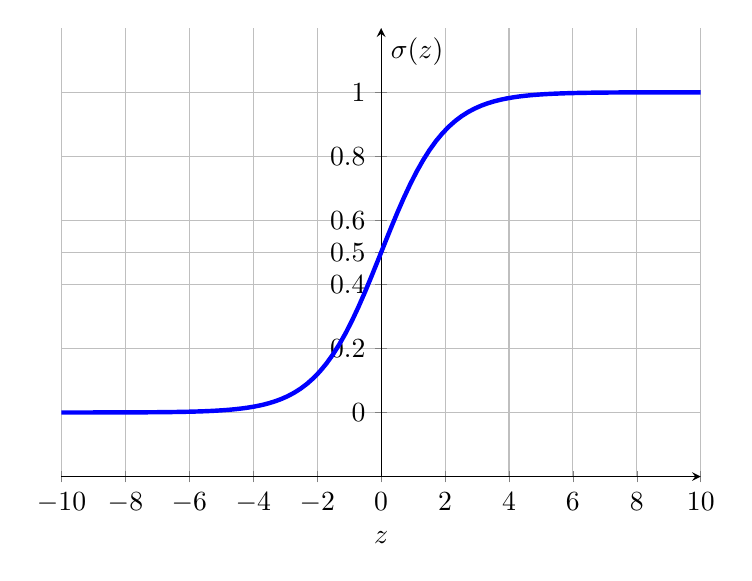
\begin{tikzpicture}
\begin{axis}
[
    grid=major,   
    xmin=-10,
    xmax=10,
    axis x line=bottom,
    ytick={0,.2,.4,.5,.6,.8,1},
    ymax=1.2,
    ymin=-0.2,
    axis y line=middle,
    width=0.8\textwidth,
    height=0.6\textwidth,
    xlabel={$z$},
    ylabel={$\sigma(z)$}
]
    \addplot%
    [
        blue,%
        mark=none,
        samples=100,
        domain=-10:10,
        ultra thick
    ]
    (x,{1/(1+exp(-x))});
\end{axis}
\end{tikzpicture}
    \caption{Plot of sigmoid function $\sigma(z)$.}
      \label{fig:sigmoid}
\end{figure}
%As seen in Figure \ref{fig:sigmoid}, $\sigma(z) \geq 0.5$ when $z \geq 0$. This means that if the linear predictor $z$ has a value greater than 0, the posterior probability of observing the class label $c=1$ is greater than 0.5, thus we would assign the class label $c=1$. 
The parameters are learned during training using the maximum likelihood estimation method. For each training instance $(d_i|c_i)$, the probability of observing the class label $c_i$ given the parameters $(w,b)$ is calculated. Assuming independence among training instances, these probabilities can be multiplied to a single equation, shown in Equation \eqref{eq:logistic_max} \cite{DBLP:books/aw/TanSKK2019}:
        \begin{equation}
        \begin{split}
            \label{eq:logistic_max}
                L(w,b) & = \prod_{i=1}^{n}P(c_i|d_i,w,b), \\
                        & = \prod_{i=1}^{n}P(y=1|x_i)^{y_i} * P(y=0|x_i)^{1-y_i}, \\
                    &    = \prod_{i=1}^{n}(\sigma(w^T x_i + b))^{y_i} * (1 - \sigma(w^T x_i + b))^{1-y_i}.
                        \end{split}
        \end{equation}
Using the likelihood of all training instances $L(w,b)$, the parameters $(w*,b*)$ with the maximum likelihood are chosen. Hence, the sigmoid function and thus the posterior probabilities $P(c=1|d)$ and $P(c=0|d)$ can be estimated and the document classified \cite{DBLP:books/aw/TanSKK2019}.


\subsubsection{Support Vector Machine}
Tan et al. define the Support Vector Machine as a discriminative classifier. It is based on a separating hyperplane that, as the name suggests, tries to separate instances of two classes. Furthermore, it only uses a subset of the training instances, those nearest the borders and thus hardest to classify. These instances are called support vectors \cite{DBLP:books/aw/TanSKK2019}.

The hyperplane can be described by Equation \eqref{eq:hyperplane}:
    \begin{equation}
            \label{eq:hyperplane}
                w^Td + b = 0,
        \end{equation}
    where $d$ represents the attributes and $(w, b)$ are the parameters of the model \cite{DBLP:books/aw/TanSKK2019}. 
    
    There can be an indefinite number of hyperplanes, which is why it is necessary to choose one that has good generalization performance, which means that it can handle unseen instances. To do this, the margin of a hyperplane $B_i$ is calculated by drawing two hyperplanes, $B_i1$ and $B_i2$, parallel to $B_i$. The distance between the two hyperplanes is the margin of the hyperplane $B_i$, as seen in Figure \ref{fig:svm} \cite{DBLP:books/aw/TanSKK2019}. By choosing the hyperplane with the maximum margin, the classifier can allow for slight changes in data without immediately crossing onto the other side.

    \begin{figure}
        \centering
        \caption{Margin of a hyperplane in a two-dimensional data set by Tan et al. \cite{DBLP:books/aw/TanSKK2019}.
        \label{fig:svm}
        }
        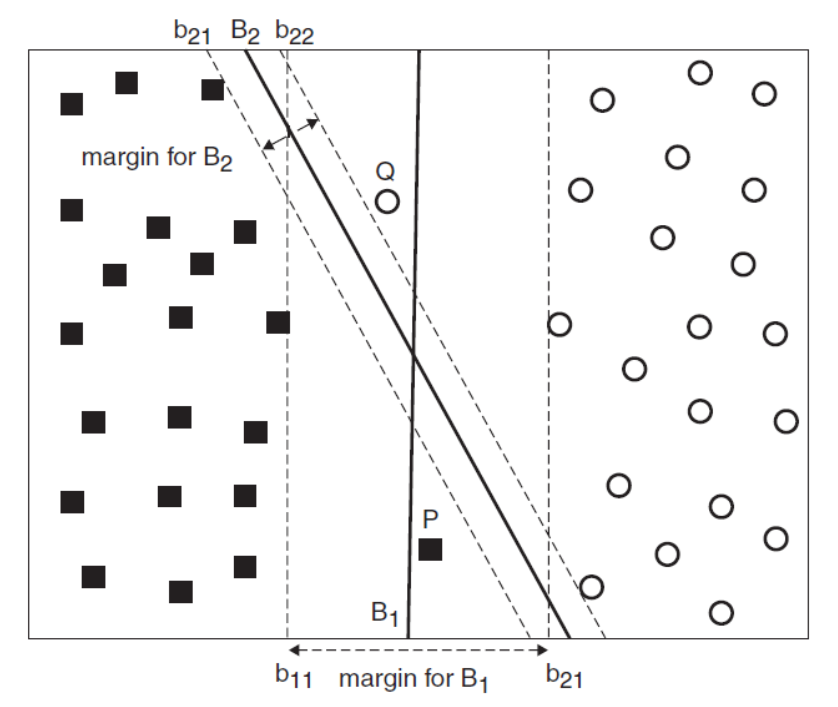
\includegraphics[scale=0.7]{Images/SVM_image.png}
    \end{figure}
    

    In Figure \ref{fig:svm}, the data can be separated by a linear hyperplane. This is not always the case, which is why a nonlinear Support Vector Machine transforms its input data $x$ into a new attribute space $\phi(x)$, in which a linear hyperplane can be constructed. Projected into the original attribute space, this hyperplane is a nonlinear decision boundary \cite{DBLP:books/aw/TanSKK2019}.
    